\documentclass[10pt,twocolumn,letterpaper]{article}
\usepackage{cvpr}
\usepackage{times}
\usepackage{graphicx}
\usepackage{amsmath}
\usepackage{amssymb}
\usepackage[pagebackref=true,breaklinks=true,colorlinks,bookmarks=false]{hyperref}
\graphicspath{ {./} }

\def\GroupID{G01} % <------- ENTER YOUR COMP 6321 group number here

\begin{document}
\title{News Classification Models}
\author{Giselle Martel ID26352936 \and Firas Sawan ID26487815}
\maketitle

\begin{abstract}
   Abstract here. Give an executive summary of your report: rough goal, rough methods, rough results. Usually no more than 200 words.
\end{abstract}

%------------------------------------------------------------------------
\section{Introduction}
\textcolor{blue}{State your goal by giving give an example of the data you're working with and an example of the kind of prediction you hope to achieve. Don't bother with a literature review of your subject area, but do mention any important sources you directly relied upon.}\\

The term “fake news” mainly refers to false or inaccurate information that is mistakenly or inadvertently created or spread. Fake news may have some hints of truth, but lack any contextualizing details. They may not include any verifiable facts or sources or may include basic verifiable facts that are written using deliberately inflammatory language that leaves out pertinent details or only presents one viewpoint. Our project aims to analyze and classify a list of news articles from 2 different datasets containing fake news and Real news entries. Entries in both datasets have a similar structure and are of the following form:   

\begin{center}
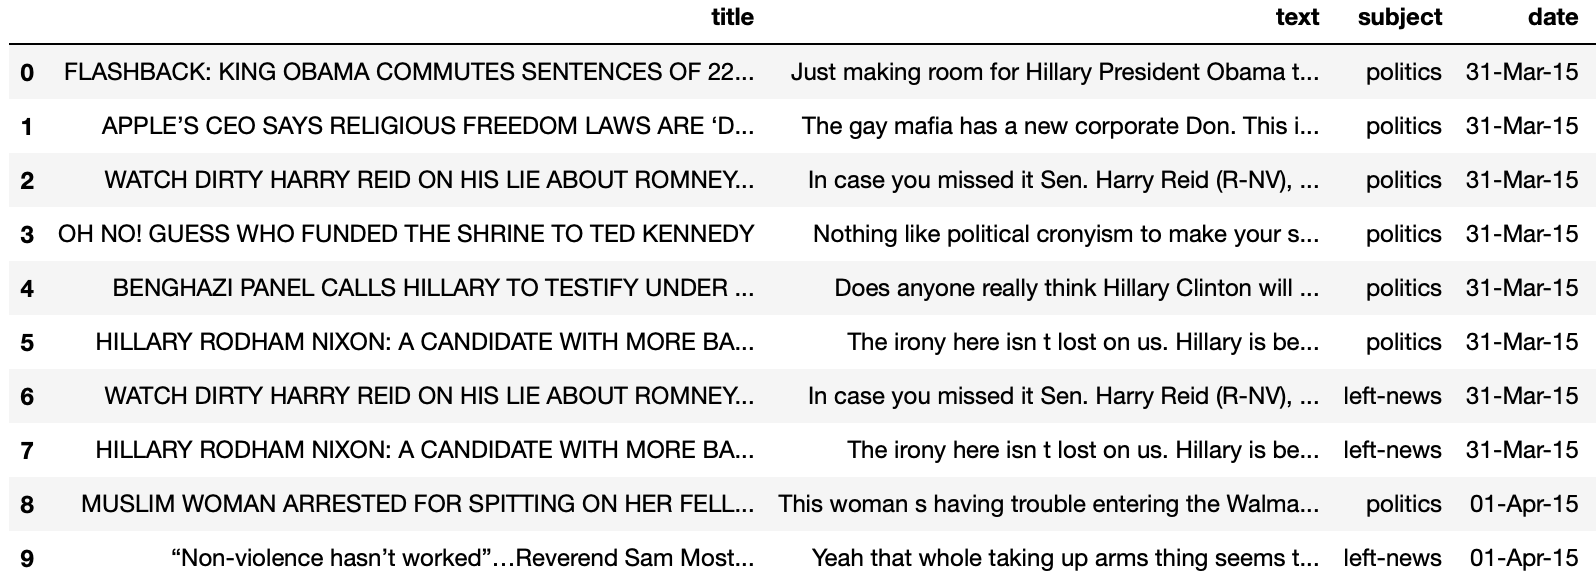
\includegraphics[width=\linewidth]{project_guide/report/dt_example.png}
\end{center}

The datasets were retrieved from a similar experiment conducted by (insert author here) however, the implementation details of the experiment have been thoroughly modified and expanded. The basic organization of the datasets include a title for each article, the text of the article, its subject and its date. Our project aims to classify words from these articles into two categories, namely a fake news category and a true news category by predicting the probability that a particular word is in present in either a fake or true news article. This classification and prediction is to be made using machine learning models that we have learned in class, namely a Support Vector Machine Classifier, a Random Forest Classifier, a Decision Tree Classifier, a Multinomial Naive Bayes Classifier, a Logistic regression Classifier, and A convolutional neural network. \\

The results we aim to achieve are in the form of detailed graphs and confusion matrices for each of the classifiers as well as a report of accuracy, percision and recall metrics. 


%------------------------------------------------------------------------
\section{Methodology \& Experimental Results}

\textcolor{blue}{Describe the important steps you took to achieve your goal, alongside experimental results that followed. If certain steps (preprocessing, extra features, etc.) turned out to be important for maximizing prediction performance, then try to mention how much benefit you observed with/without that feature.}

The first step we had to take to prepare for our experiment was to preprocess our data. This was an important step given that we needed maximize prediction performance by getting rid of empty data cells as well as formatting all entries in each column of both datasets in a similar manner. Preprocessing the data involved parsing both datasets, clearing out empty data cells, formatting the date columns in a uniform manner for all cells. It also involved assigning each dataset their respective labels of fake vs true news. Once this was done  both files were joined together to create one big dataset that we later used in our tokenization process. Tokenization was a necessary process that allowed us to extract all unique words from the joined dataset in preparation for splitting the data into training and testing components. We opted to split the data into a 70\% training set and a 30\% testing set as it seemed ideal to have our training data consisting of more than double that of the testing data. Following the split we generated a document-term matrix for each of the training and testing data and converted both the testing and training datasets into dataframes that we later used in our models. \\

The first model we  worked on was the Multinomial Naive Bayesian model given that it is suitable for classification of discrete features such as the tokenized text in our preprocessed dataset. We used the corresponding sklearn library to generate our model and fit our data to that model and then made the predictions, generated a confusion matrix and displayed a graph as shown below:

\begin{center}
\includegraphics[width=\linewidth]{}
\end{center}

The model successfully achieved an accuracy of (insert accuracy) and a confusion matrix that helped in visualizing the classification results of this model.\\ 

Next, we worked on the Decision Tree classifier with the goal of creating a supervised learning model that predicts the correct label for a particular word by learning simple decision rules inferred from the training data features. We used the corresponding Sklearn library to create our model and passed a max\_depth parameter of 5000 and fit our data to it in order to generate the necessary predictions shown below: 

\begin{center}
\includegraphics[width=\linewidth]{}
\end{center}

The model successfully achieved an accuracy of (insert accuracy) and the confusion matrix shown above that helped in visualizing the classification results of this model.\\ 

Next, we worked on the Random Forest classifier that fits a number of decision tree classifiers on various sub-samples of the dataset and uses averaging to improve the predictive accuracy while controlling over-fitting to a satisfying degree. We used the corresponding Sklearn library to generate our model and with the help of the GridSearchCV method we performed an exhaustive search over specified parameter values for our estimator. The parameter values used, namely the depth and the number of estimators, were chosen experimentally to ensure optimal performance of our model. Next we fit our data to the model and then made the predictions shown below:

\begin{center}
\includegraphics[width=\linewidth]{}
\end{center}

The model successfully achieved an accuracy of (insert accuracy) and the confusion matrix shown above helped in visualizing the classification results of this model.\\ 

A Support Vector Machine model, which is a form of supervised learning, was then used to further help us in our quest for category prediction and classification. This model had an advantage of being memory efficient in the sense that it uses a subset of training points in the decision function called support vectors. In terms of the parameters used, we chose a Gaussian kernel of type 'rbf' and decided to implement a custom hyper parameter search that allowed us to obtain the best possible parameters for this model. We report the accuracy of this model and a confusion matrix that helps visualize the classification results obtained using this model: 

\begin{center}
\includegraphics[width=\linewidth]{}
\end{center}

The model successfully achieved an accuracy of (insert accuracy) and the confusion matrix shown above that helped in visualizing the classification results of this model.\\ 

Next, we worked on a Logistic Regression model that we used to predict the probability of our categorically dependent variables. We used the corresponding Sklearn library to generate our model and fit our data to it. The model worked in such a way that it treated our tokenized data as binary variables that contain data coded as 1 (in our case Real) or 0 (in our case "fake") and used this data to make predictions. We reported the accuracy of this model and a confusion matrix obtained: 

\begin{center}
\includegraphics[width=\linewidth]{}
\end{center}

The model successfully achieved an accuracy of (insert accuracy) and the confusion matrix shown above that helped in visualizing the classification results of this model.\\ 

Finally, a neural network was constructed 

%------------------------------------------------------------------------
\section{Conclusions}

Summarize what you could and could not conclude based on your experiments.

The "References" section (bibliography) is optional. If you cite any books, websites, or academic papers, then you can add them to bibliography.bib and cite them in this report. Otherwise delete the references section.


{\small
\bibliographystyle{cvpr_bibstyle}
\bibliography{bibliography}
}


\newpage
\appendix


%-------------------------------------------------------------------------
\section*{Appendix: Extra Results (Optional)}

% DELETE THIS TEXT
If you want to include extra more detailed results that did not fit within the main report, include them here. Or, you can just delete this example section.

%-------------------------------------------------------------------------
\section*{Appendix: Examples of \LaTeX}

% The 'dilde' in Table~\ref{} puts a no-break space prevents "Table" and "1" so that
% the table number does not get split onto a separate line.
% and it is good LaTeX practice to put tildes between 

% DELETE THIS TEXT
This section contains some examples of \LaTeX~to help you get started.
(You should delete this section in the final report.)
This is a reference to Table~\ref{first_table} and Table~\ref{second_table}.
This is a reference to Figure~\ref{first_figure} and Figure~\ref{second_figure}.
This is a citation \cite{breiman2001statistical} and this is
multiple citations \cite{breiman2001statistical,bishop2006pattern}.
This is \textit{italics} and \textbf{bold} text.
This is a formula $\sum_{i=1}^N (y_i - \hat{y}_i(\mathbf{x}))^2$
that is inline with the text (`text style') and this is a
formula that is displayed separately (`display style'):
$$
\sum_{i=1}^N (y_i - \hat{y}_i(\mathbf{x}))^2
$$
These are formulas with an associated equation number
\begin{align}
   \mathbf{x} = \begin{bmatrix}
      x_1, x_2, \ldots, x_N
   \end{bmatrix}^T    \label{xvec}\\
   \boldsymbol{\phi} = \begin{bmatrix}
      \phi_1, \phi_2, \ldots, \phi_M
   \end{bmatrix}^T    \label{phivec}
\end{align}
and we can now refer back to~\eqref{xvec} or to ~\eqref{phivec} like so.



% DELETE THIS TABLE
\begin{table}
   \begin{center}
   \begin{tabular}{|l|c|c|}
   \hline
   Method & Ultra-Clustering & Random Jungles \\
   \hline\hline
   Theirs & Works OK & All your base\\
   Yours & Works better & are belong to us!\\
   Ours & Works best! & I can haz publication?\\
   \hline
   \end{tabular}
   \end{center}
   \caption{This is the caption of a column-width table.\label{first_table}}
\end{table}

% DELETE THIS TABLE
\begin{table*}
   \begin{center}
   \begin{tabular}{|l|c|c|c|}
   \hline
   Method & Good? & Bad? & So-so? \\
   \hline\hline
   Your method & Terrible & Yes, I made sure of it & Star Wars movies \\
   My supervisor's old method (sigh) & I want Tim Horton's & People in hallway... & ...are talking too loudly \\
   My proposed method  & Yes, good! & No, I said good! & What? \\
   \hline
   \end{tabular}
   \end{center}
   \caption{This is the caption of a page-width table.\label{second_table}}
\end{table*}


% DELETE THIS FIGURE
\begin{figure}
   \begin{center}
   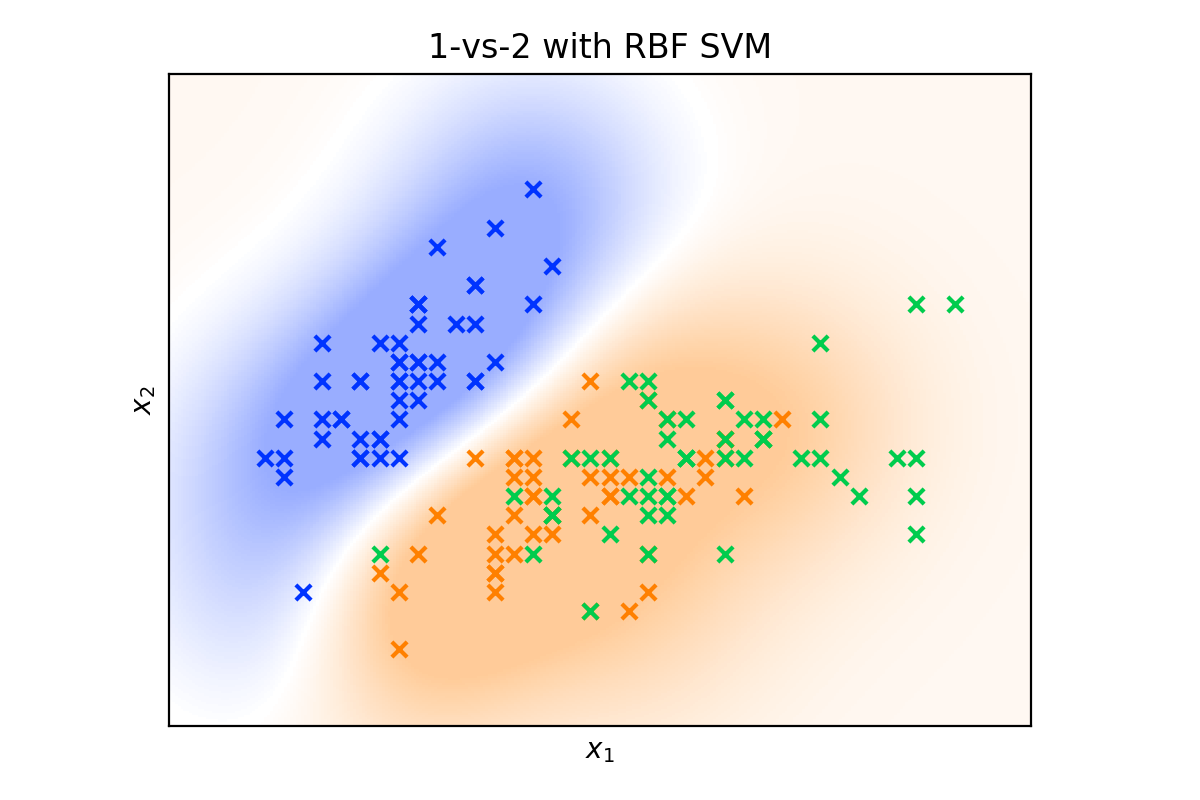
\includegraphics[width=\linewidth]{sample_image.png}
   \end{center}
      \caption{This is the caption of a column-width figure.\label{first_figure}}
\end{figure}
   

% DELETE THIS FIGURE
\begin{figure*}
   \begin{center}
      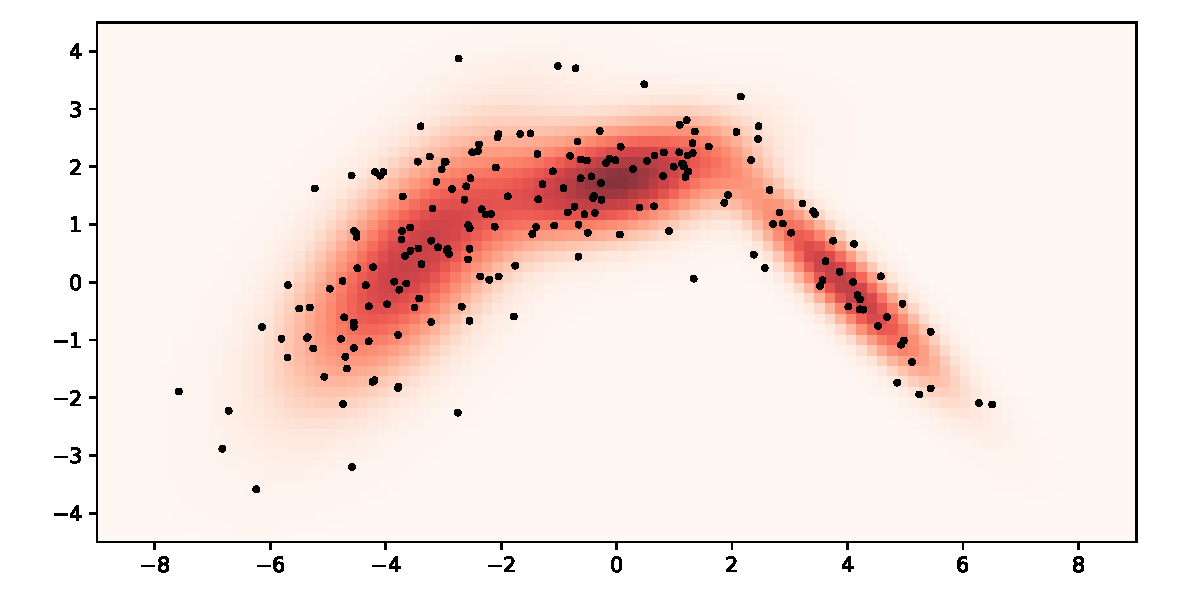
\includegraphics[width=0.4\linewidth]{sample_image.pdf}
      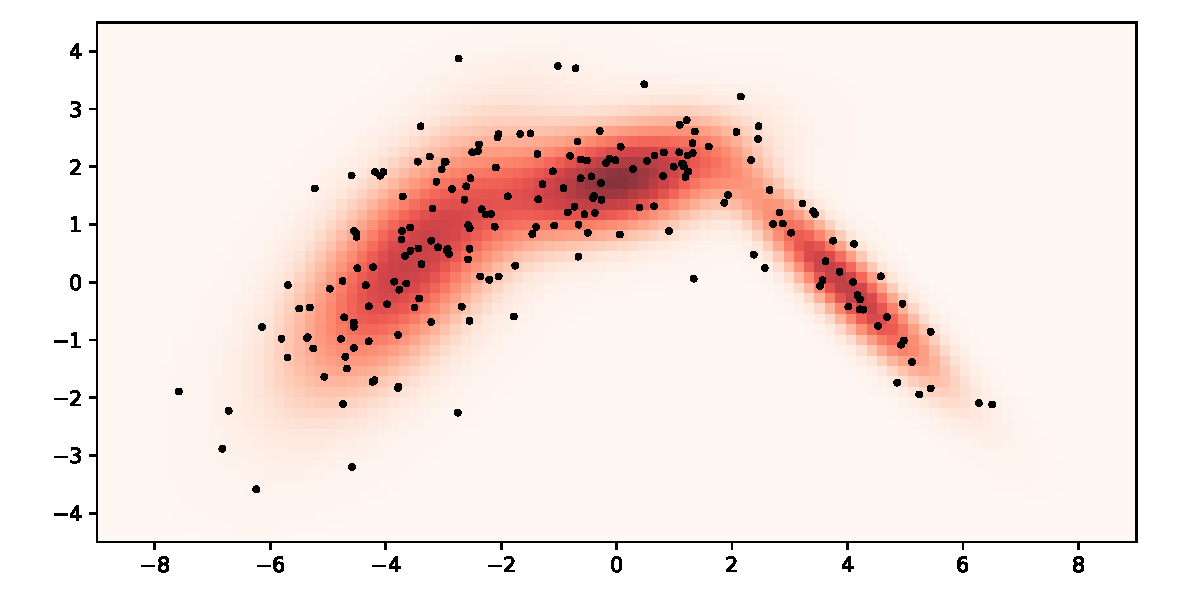
\includegraphics[width=0.4\linewidth]{sample_image.pdf}
   \end{center}
      \caption{This is the caption of a page-width figure.\label{second_figure}}
\end{figure*}




\end{document}
